\documentclass{article}

\usepackage{graphicx}
\usepackage{tikz}
\usepackage{tikzsymbols}
\usetikzlibrary{calc,patterns,shapes.geometric}
\pagestyle{empty}
\usepackage[margin=0pt]{geometry}
\geometry{papersize={14in,12in}}

\def\centerarc[#1](#2)(#3:#4:#5){\draw[#1] ($(#2)+({#5*cos(#3)},{#5*sin(#3)})$) arc (#3:#4:#5);}

\begin{document}
	\begin{figure}
		\centering
		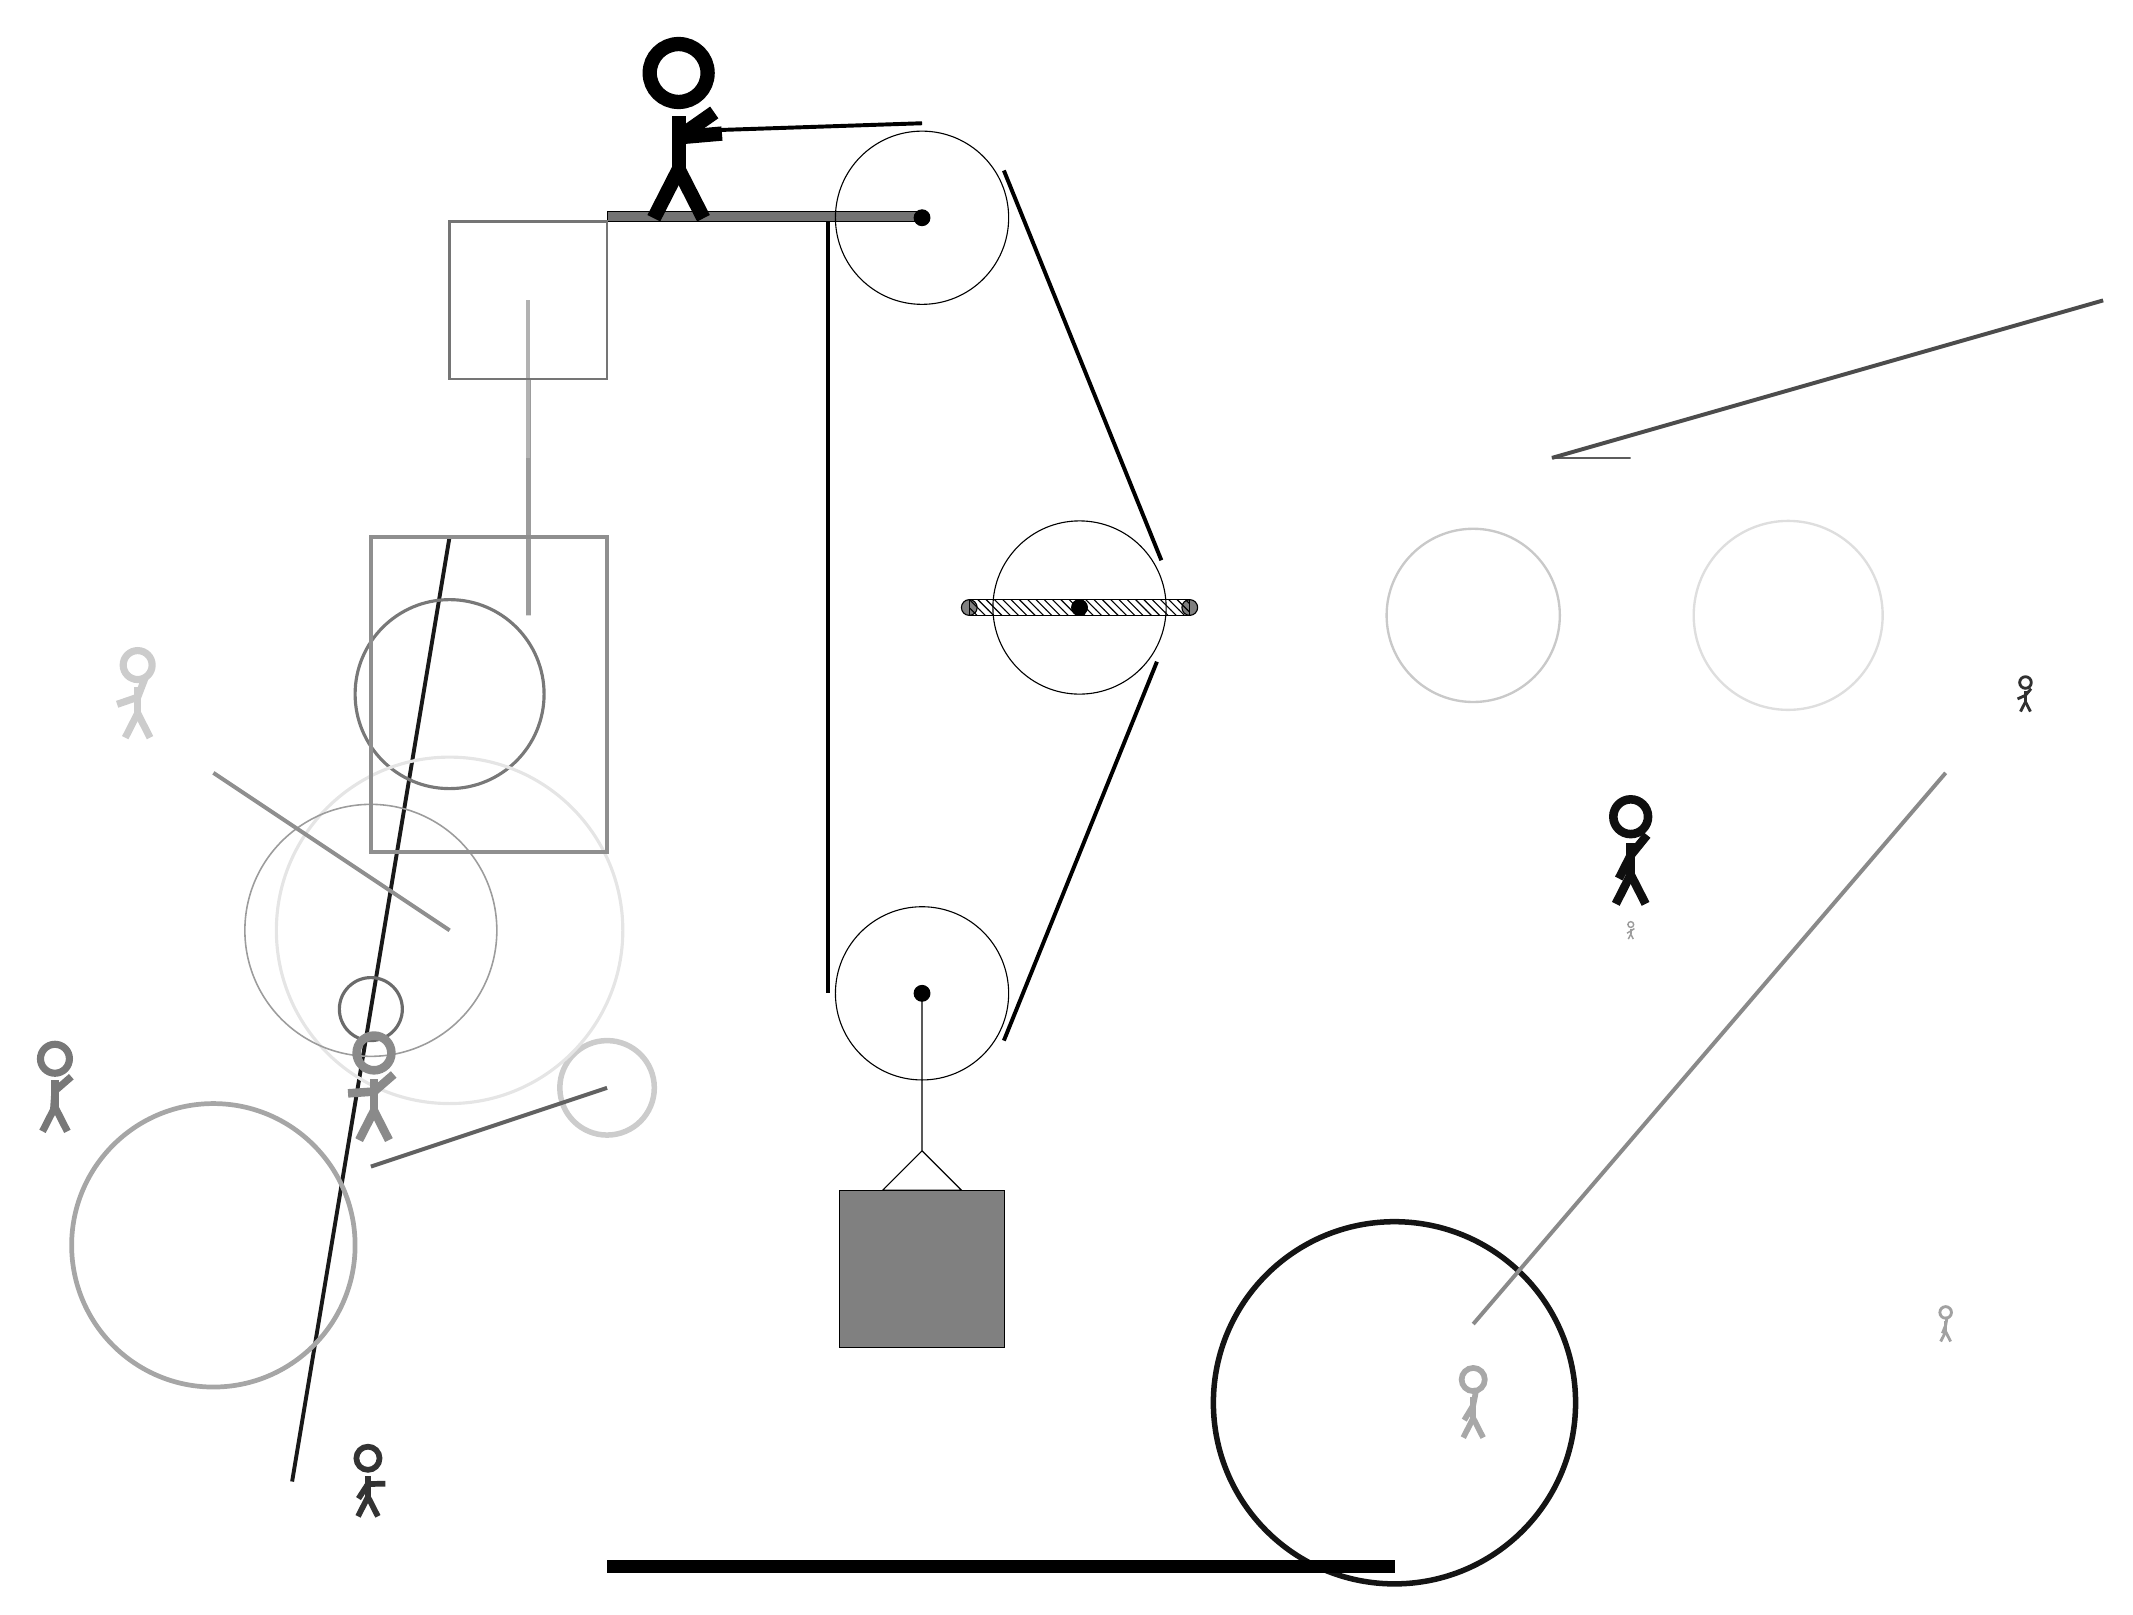
\begin{tikzpicture}
			%%%%% START %%%%%
			
			\draw[fill=black!55] (-2, 14) rectangle (2, 14.125);
			
			\draw (2, 4.2) circle (1.1);
			\draw[fill=black] (2, 4.2) circle (0.1);
			
			\draw (2, 14.05) circle (1.1);
			\draw[fill=black] (2, 14.05) circle (0.1);
			
			\draw[fill=white](4, 9.1) circle (1.1);
			\draw[fill=black] (4, 9.1) circle (0.1);
			\draw[fill=black!50] (2.6, 9.1) circle (0.1);
			\draw[fill=black!50] (5.4, 9.1) circle (0.1);
			\draw[pattern=north west lines, pattern color=black] (2.6, 9.2) rectangle (5.4, 9.0);
			
			\draw (2, 4.2) -- (2, 2.2) -- (1.5, 1.7) -- (2.5, 1.7) -- (2, 2.2);
			\draw[fill=black!50] (0.95, 1.7) rectangle (3.05, -0.3);
			
			\draw[line width=0.5mm] (0.8, 14) -- (0.8, 4.2);
			\centerarc[line width=0.5mm](2, 4.2)(180:330:1.2000000000000002);
			\draw[line width=0.5mm](3.0392, 3.6) -- (4.983, 8.4117);
			\centerarc[line width=0.5mm](4, 9.1)(390:325:1.2000000000000002);
			\draw[line width=0.5mm](5.0392, 9.7) -- (3.0392, 14.65);
			\centerarc[line width=0.5mm](2, 14.05)(30:90:1.2000000000000002);
			\draw[line width=0.5mm](2, 15.25) -- (-1, 15.15);
			
			\node at (-1, 15.15) {\Strichmaxerl[10][-175][35]};
			
			\draw[line width=0.6mm, color=black!39] (-3, 9) rectangle (-3, 12);
			
			\node[line width=0.3mm, color=black!94] at (11, 6) {\Strichmaxerl[6][63][51]};
			\draw[line width=0.5mm, color=black!90](-6, -2) -- (-4, 10);
			\node[line width=0.2mm, color=black!53] at (-9, 3) {\Strichmaxerl[5][86][41]};
			\draw [line width=0.4mm, color=black!58](-5, 4) circle (0.4);
			\draw[line width=0.5mm, color=black!30](-3, 11) -- (-3, 13);
			\node[line width=0.7mm, color=black!80] at (-5, -2) {\Strichmaxerl[4][57][1]};
			\draw[line width=0.3mm, color=black!64] (10, 11) rectangle (11, 11);
			\draw [line width=0.7mm, color=black!20](-2, 3) circle (0.6);
			
			\draw[line width=0.5mm, color=black!62](-5, 2) -- (-2, 3);
			\draw [line width=0.4mm, color=black!53](-4, 8) circle (1.2);
			
			\draw [line width=0.3mm, color=black!21](9, 9) circle (1.1);
			\draw [line width=0.4mm, color=black!10](-4, 5) circle (2.2);
			
			\draw [line width=0.3mm, color=black!13](13, 9) circle (1.2);
			\node[line width=0.2mm, color=black!81] at (16, 8) {\Strichmaxerl[2][24][50]};
			\draw[line width=0.5mm, color=black!70](10, 11) -- (17, 13);
			
			\draw[line width=0.5mm, color=black!45](-5, 3) -- (-5, 3);
			
			\draw [line width=0.2mm, color=black!39](-5, 5) circle (1.6);
			\node[line width=0.5mm, color=black!46] at (-5, 3) {\Strichmaxerl[6][4][41]};
			\draw[line width=0.3mm, color=black!54] (-2, 14) rectangle (-4, 12);
			\node[line width=0.6mm, color=black!37] at (15, 0) {\Strichmaxerl[2][68][80]};
			
			\draw [line width=0.7mm, color=black!92](8, -1) circle (2.3);
			
			\draw[line width=0.5mm, color=black!46](9, 0) -- (15, 7);
			\node[line width=0.7mm, color=black!20] at (-8, 8) {\Strichmaxerl[5][19][69]};
			\node[line width=0.2mm, color=black!34] at (9, -1) {\Strichmaxerl[4][59][79]};
			\draw[line width=0.5mm, color=black!44] (-2, 6) rectangle (-5, 10);
			\draw[line width=0.5mm, color=black!44](-7, 7) -- (-4, 5);
			\node[line width=0.5mm, color=black!39] at (11, 5) {\Strichmaxerl[1][30][34]};
			\draw [line width=0.6mm, color=black!35](-7, 1) circle (1.8);
			
			\draw[fill=black] (-2, -3) rectangle (8, -3.15);
			
			%%%%% END %%%%%
		\end{tikzpicture}
	\end{figure}	
\end{document}